\newpage
\section{Results}

This section presents the results and their respective conclusion on all the experiments and their preliminary tests.

\subsection{Girvan-Newman approximation}


\textbf{Preliminary test}

The results of the semi-supervised classification task on the CORA dataset are show on the following table:


\begin{table}[H]
\centering
\begin{tabular}{|llccc|c}
%\toprule
\hline
    Model &           params &   Val Loss &   Test Accuracy &   Duration \\
%\midrule
\hline
   SGConv &   100\_epochs=200 &     1.7587 &   0.790 ± 0.018 &      0.585 \\
 ChebConv &   100\_epochs=200 &     0.8133 &   0.769 ± 0.027 &      5.049 \\
    APPNP &   100\_epochs=200 &     0.8894 &   0.808 ± 0.017 &      0.984 \\
  GATConv &   100\_epochs=200 &     0.8111 &   0.803 ± 0.016 &      1.967 \\
  GCNConv &   100\_epochs=200 &     0.8864 &   0.789 ± 0.018 &      1.091 \\
%\bottomrule
\hline
\end{tabular}
\label{preliminar_GN}\caption{Reproduced benchmark semi-supervised classification experiments on CORA dataset }
\end{table}

We observe that test accuracy is correct in all the models trained, successfully replicating the experiments. Setup of the environment is also correctly verified.




\textbf{Main experiment}

As detailed in the experiments section, the main experiment is to train a model to approximate the edge betweenness of part of the edges of a graph, in a semi-supervised manner. The performance is measured with the accuracy and F1-score macro averaged after transforming the edge betweenness values into a finite number of ranges (bucketization or discretization). Different number of discrete ranges have been tested and using 28 ranges is the most optimal. For generating the buckets(discrete ranges) the function qcut from Pandas Python library has been used to split the data by the desired number of percentiles. The results are shown in the following table:

% \begin{table}[H]
% \centering
% \begin{tabular}{|llllccc|}
% \hline
%  Model &                                                                        Parameters  &  Runs\/Epochs  &  Splits &    Loss &        Accuracy &  Time(min) \\
% \hline
%  META1 &          d19d16h10e19n16n15 & 1-2 & 20-500-1500 &  1.6367 &     0.239  &      0.069 \\
%  META2 &       d19d16h10e19n16n15 & 100-20 & 20-500-1500 &  1.7550 &   0.296 ± 0.031 &      0.494 \\
%  META3 &      d19d16h10e19n16n15 & 100-200 & 20-500-1500 &  2.7132 &   0.274 ± 0.019 &      3.518 \\
%  META4 &      d19d16h10e19n16n15 & 100-20 & 20-500-10556 &  1.7508 &   0.293 ± 0.023 &      0.547 \\
%  META5 &     d19d16h10e19n16n15 & 100-200 & 20-500-10556 &  2.8676 &   0.266 ± 0.013 &      3.743 \\
%  META6 &     d19d16h10e19n16n15 & 100-20 & 20-4000-10556 &  1.7437 &   0.296 ± 0.026 &      0.528 \\
%  META7 &    d19d16h10e19n16n15 & 100-200 & 20-4000-10556 &  2.8105 &   0.265 ± 0.016 &      3.704 \\
%  META8 &    d19d16h10e19n16n15 & 100-20 & 300-4000-10556 &  1.1625 &   0.563 ± 0.067 &      0.506 \\
%   META1 &   d19d16h10e19n16n15 & 100-20 & 300-4000-10556- &  0.9832 &   \textbf{0.621 ± 0.069} &      0.408 \\
%  META9 &   d19d16h10e19n16n15 & 100-200 & 300-4000-10556 &  2.3160 &   0.409 ± 0.033 &      3.546 \\
%  META10 &    d10d10h10e10n10n10 & 100-20 & 300-4000-10556 &  1.1565 &   0.537 ± 0.074 &      0.494 \\
%  META11 &   d10d10h10e10n10n10 & 100-200 & 300-4000-10556 &  2.1036 &   0.374 ± 0.030 &      3.593 \\
 
% \hline
% \end{tabular}
% \label{Experiment1}\caption{Edge betweenness approximation with a graph neural network experiment using 5 discrete ranges}
% \end{table}


% For increasing the number of buckets(discrete ranges) the function qcut from Pandas Python library has been used to be able to split the data by the desired number of percentiles.

% \begin{table}[H]
% \centering
% \begin{tabular}{|llllccc|}
% \hline
%  Model &  Parameters  &  Runs\/Epochs  &  Splits &    Loss &        Accuracy &  Time(min) \\
% \hline
%  META1 &        d19d16h10e19n16n15 & 100-20 & 20-500-1500- &  3.0321 &   0.136 ± 0.022 &      0.512 \\
%  META1 &        d19d16h10e19n16n15 & 100-50 & 20-500-1500- &  3.3168 &   0.116 ± 0.021 &      0.959 \\
%  META1 &       d19d16h10e19n16n15 & 100-100 & 20-500-1500- &  3.7570 &   0.107 ± 0.020 &      1.800 \\
%  META1 &       d19d16h10e19n16n15 & 100-200 & 20-500-1500- &  4.5076 &   0.094 ± 0.014 &      3.585 \\
%  META1 &       d19d16h10e19n16n15 & 100-250 & 20-500-1500- &  4.8326 &   0.089 ± 0.014 &      4.439 \\
%  META1 &       d19d16h10e19n16n15 & 100-300 & 20-500-1500- &  5.3309 &   0.083 ± 0.013 &      5.290 \\
%  META1 &       d19d16h10e19n16n15 & 100-350 & 20-500-1500- &  5.2242 &   0.088 ± 0.015 &      6.054 \\
%  META1 &       d19d16h10e19n16n15 & 100-400 & 20-500-1500- &  5.7016 &   0.083 ± 0.014 &      6.846 \\
%  META1 &       d19d16h10e19n16n15 & 100-450 & 20-500-1500- &  5.9954 &   0.082 ± 0.013 &      7.720 \\
%  META1 &       d19d16h10e19n16n15 & 100-550 & 20-500-1500- &  6.2228 &   0.084 ± 0.013 &      9.396 \\
%  META1 &       d19d16h10e19n16n15 & 100-600 & 20-500-1500- &  6.5450 &   0.081 ± 0.012 &     10.338 \\
%  META1 &       d19d16h10e19n16n15 & 100-650 & 20-500-1500- &  6.5845 &   0.082 ± 0.014 &     11.119 \\
% \hline
% \end{tabular}
% \label{Experiment1}\caption{Edge betweenness approximation with a graph neural network experiment using 28 discrete ranges}
% \end{table}


% The best models obtain have a respective maximum accuracy of is 62.3\% in the 5 discrete ranges setup and 8.1\% in the 28 discrete ranges setup. The second model is selected by looking at the scatter plot of predicted versus real values. The following plots show the distribution of predicted values compared to the real values, both for the discrete and real values.

\begin{table}[H]
\centering
\begin{tabular}{|llllccc|}
\hline
 Model &                                                                          Paramteres  &  Runs\/Epochs  &  Splits &    Loss &        Accuracy &        F1-macro  \\
\hline
 META1 &      d19d16h10e19n16n15 & 100-20 & 100-2000-10556- &  2.3561 &   0.280 ± 0.061 &   0.251 ± 0.060  \\
 META1 &     d19d16h10e19n16n15 & 100-250 & 100-2000-10556- &  3.8995 &   0.139 ± 0.018 &   0.128 ± 0.020  \\
 META1 &         d19d16h10e19n16n15 & 100-20 & 20-500-1500- &  3.0269 &   0.142 ± 0.027 &   0.127 ± 0.029  \\
 META1 &        d19d16h10e19n16n15 & 100-250 & 20-500-1500- &  4.9482 &   0.093 ± 0.013 &   0.087 ± 0.017  \\
 META1 &      d19d16h10e19n16n15 & 100-20 & 200-3000-10556- &  2.0677 &  \textbf{ 0.342 ± 0.078} &   \textbf{0.312 ± 0.076 } \\
 META1 &     d19d16h10e19n16n15 & 100-250 & 200-3000-10556- &  3.3414 &   0.219 ± 0.027 &   0.208 ± 0.028  \\
 META1 &    d19d16h10e19n16n15 & 100-600 & 200-3000-10556- &  3.7691 &   0.142 ± 0.037 &   0.124 ± 0.039  \\
 META1 &    d19d16h10e19n16n15 & 100-2 & 20-500-10556- &  3.0165 &   0.112 ± 0.047 &   0.088 ± 0.052 \\
\hline
\end{tabular}
\label{Experiment1-v2}\caption{Edge betweenness approximation with a graph neural network experiment using 28 discrete ranges}
\end{table} 




% \begin{figure}[H]
% \minipage{0.5\textwidth}%
%   \centering
%     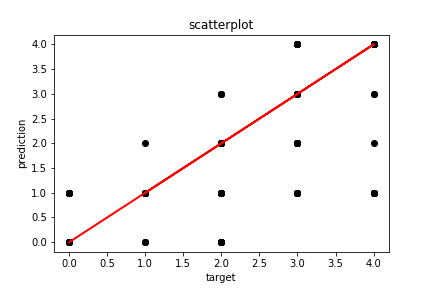
\includegraphics[width=0.9\linewidth]{img/GN_exp1/2019-09-28_22-02-07_META1_d4=19_d5=16_hus=10_eus=19_n1us=16_n2us=15_r=100_epochs=20_split-300-4000-10556-_scatterplot.png}
% \endminipage
% \minipage{0.5\textwidth}%
%   \centering
%     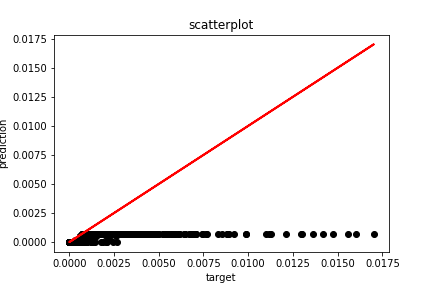
\includegraphics[width=0.9\linewidth]{img/GN_exp1/2019-09-28_22-02-07_META1_d4=19_d5=16_hus=10_eus=19_n1us=16_n2us=15_r=100_epochs=20_split-300-4000-10556-_scatterplot_real_eb.png}
% \endminipage
% \caption{Scatter plot comparing target edge betweenness and predicted (discrete range and real values)}\label{fig:edgeb_exp1_scatter}
% \end{figure}


% \begin{figure}[H]
% \minipage{0.5\textwidth}%
%   \centering
%     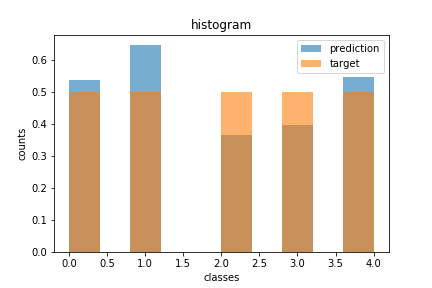
\includegraphics[width=0.9\linewidth]{img/GN_exp1/2019-09-28_22-02-08_META1_d4=19_d5=16_hus=10_eus=19_n1us=16_n2us=15_r=100_epochs=20_split-300-4000-10556-_histogram.png}
% \endminipage
% \minipage{0.5\textwidth}%
%   \centering
%     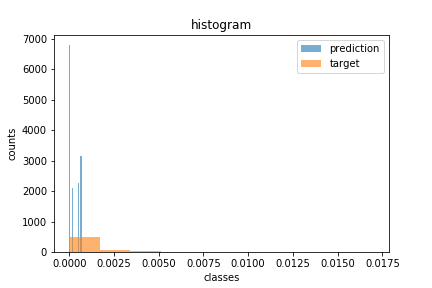
\includegraphics[width=0.9\linewidth]{img/GN_exp1/2019-09-28_22-02-08_META1_d4=19_d5=16_hus=10_eus=19_n1us=16_n2us=15_r=100_epochs=20_split-300-4000-10556-_histogram_real_eb.png}
% \endminipage
% \caption{histogram of target values versus predicted values of edge betweenness in both discrete and continuous display }\label{fig:edgeb_exp1_histogra}
% \end{figure}

\begin{figure}[H]
\minipage{0.32\textwidth}%
  \centering
    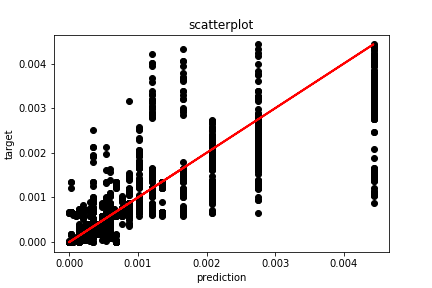
\includegraphics[width=0.9\linewidth]{img/GN_exp1/28bins/scatter_plot_20epochs.png}
\endminipage
\minipage{0.32\textwidth}%
  \centering
    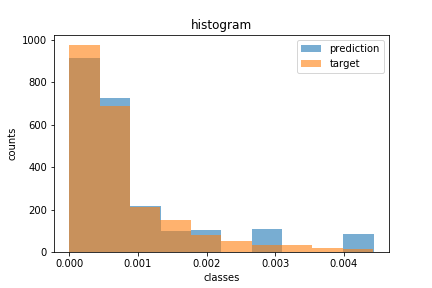
\includegraphics[width=0.9\linewidth]{img/GN_exp1/28bins/histogram_20epochs.png}
\endminipage
\minipage{0.32\textwidth}%
  \centering
    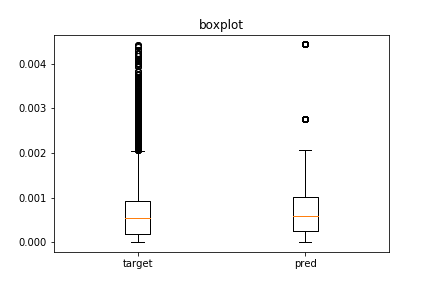
\includegraphics[width=0.9\linewidth]{img/GN_exp1/28bins/boxplot_20epochs.png}
\endminipage
\caption{Predictions compared to target values in an approximation of the edge betweenness using 28 discrete ranges and 20 epochs of training (best accuracy model) }\label{fig:edgeb_exp1_10bins}
\end{figure}


The best model is the one trained for 20 epochs, with a dataset split of 200, 3000 and 10556 train, validation and testing number of samples respectively. It attains a 34.3\% of accuracy as well as a 31.2\% f1-score macro averaged. However, when looking  into the scatter plots of predicted values versus target values, a trained model with 250 or 600 epochs seems to be better fitting the real values on some of the runs. For each model we want to train, given that the dataset split is critical to the model performance, we must run it for several times (100 in this case) and average the performance metrics to get a more realistic model performance. In the end, even if for some dataset splits the models fitted have a better performance, it is the average performance over all the splits that counts. We want the model to be able to generalize.


\begin{figure}[H]
\minipage{0.32\textwidth}%
  \centering
    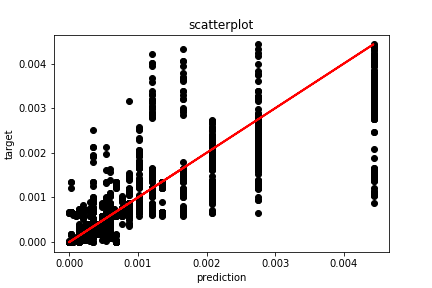
\includegraphics[width=0.9\linewidth]{img/GN_exp1/28bins/scatter_plot_20epochs.png}
\endminipage
\minipage{0.32\textwidth}%
  \centering
    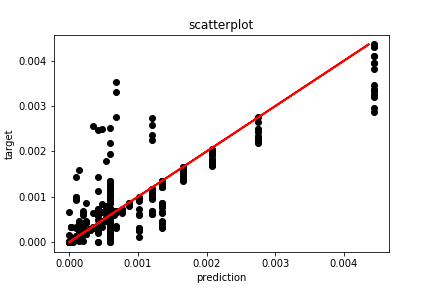
\includegraphics[width=0.9\linewidth]{img/GN_exp1/28bins/scatter_plot_250epochs.png}
\endminipage
\minipage{0.32\textwidth}%
  \centering
    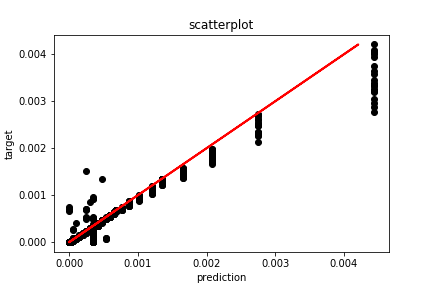
\includegraphics[width=0.9\linewidth]{img/GN_exp1/28bins/scatter_plot_600epochs.png}
\endminipage
\caption{Predictions compared to target values in an approximation of the edge betweenness using 28 ranges with 20, 250 and 650 epochs of training}\label{fig:edgeb_exp1_20bins}
\end{figure}





\textbf{Conclusion}
% conclusion on results

% value the results, how good is this accuracy vs random model
%The best models obtain have a respective maximum accuracy of is 62.3\% in the 5 discrete ranges setup and 8.1\% in the 28 discrete ranges setup.
The best trained model for predicting the edge betweenness obtains a 34.3\% of accuracy as well as a 31.2\% f1-score macro averaged in the 28 discrete ranges setup.

One important negative aspect of the models trained so far in this experiment, is that the predictive model will not predict which edge has maximum value of edge betweenness but a whole group or bucket. The final goal of the experiment is to use the model for the Girvan-Newman algorithm which needs to find the edge with highest edge betweenness. Since the model uses buckets, all edge betweennesses predicted to belong to a bucket will have all the same value. 

For the task at hand, the most important predictions are those of the edges with high edge betweenness. In that aspect, the more granular model (the one with 28 discrete ranges) is more precise and the high value predictions are less noisy than other more coarse grained models tested. A more granular model, would return a smaller set of edges that are predicted to have the highest edge betweenness, and so the subsequent tasks to refine this prediction would be faster.
% problems that this model could exhibit: higher range has more variability than others, which for finding the maximum value is problematic.


\textbf{Improvements}
% Improvements.

The first basic improvement that could be looked into is to perform a longer hyper parameter (and data partitioning configuration) search, to see if this kind of model can obtain a better accuracy. 

%It could also be trained on a larger set of buckets or classes. -> already performed


Also, it would be important to test its performance on several heterogeneous graphs, to get an idea of how stable this model training is.


%higher values for the Girvan Newman
To improve the usability for the Girvan-Newman approximation, the precision in high values should be increased. One naive solution would be to give the samples in the bucket their maximum value, because the problem is to find the real maximum and not to increase the overall values of a bucket. In one hand, to have the model to predict higher values, a smaller range with the most higher values of the training set could be created. But, since this would introduce a great deal of class imbalance, the performance of the model would decrease. This trade-off should be tested thoroughly. A good approach to solve the class imbalance would be to use a weighted loss function during the training of the Graph Neural Network. This loss would have a weight associated with the inverse of the number of samples a bucket contains. Another thing to keep in mind, is that the loss function and the error function(metric score) should be changed to something more beneficial for finding the maximal values, for example to use the f1-score of the class with highest edge betweenness value.

One different approach to this problem would be to recompute the real edge betweenness of edges predicted to belong to the highest bucket. Depending on the size of the higher bucket, this process could harm the speed of the approximation of the Girvan-Newman algorithm.

Finally, for the Girvan-Newman algorithm, an inductive setup of the graph neural network algorithm should be tested. The current transductive setup (semi-supervised learning where a few edge betweennesses will be actually computed to quickly train the model and the rest will be predicted) might impact the speed of execution. Since in each iteration some edge betweenness need to be computed, then the model needs to be trained (or fine-tuned) and then this same model is used to predict the rest of edge betweenness's, the process could be slower than the original algorithm. If a model is trained once and can directly be used in each iteration, the overall process should be faster. There is a middle ground solution, where the graph neural network model is only trained in the very first iteration of the Girvan-Newman algorithm and then in the subsequent steps it is just used for prediction. 



\newpage
\subsection{Compiled code function classification}


\textbf{Preliminary test}

The results of the graph classification task on the different datasets are show on the following table:


\begin{table}[H]
\centering
\begin{tabular}{|llccc|c}
%\toprule
\hline
    Model &         Dataset &   CV F1-macro &   Accuracy &  F1-macro \\
%\midrule
\hline
  GGNN1 &   REDDIT-BINARY   &     1.7587    &   0.75 &     0.7724 \\
  GGNN1 &   QM9             &     0.730267  &   0.8 &      0.740979 \\
  GGNN1 &   PROTEINS        &     0.735332    &   0.75 &   0.772433 \\
%\bottomrule
\hline
\end{tabular}
\label{preliminar_GN}\caption{Reproduced benchmark semi-supervised classification experiments on CORA dataset }
\end{table}

We observe that test accuracy is correct in all the models trained, successfully obtaining accuracies close to the ones in the experiments ( \cite{fey2019fast}, \cite{borgwardt2005protein}, \cite{dobson2003distinguishing}). Setup of the environment is also correctly verified. \\
\\




\textbf{Main experiment}

The next results tables show the performance of baseline  and Graph Neural Network models on the code function classification dataset in versions v1 and v3. The results are sorted by the obtained cross-validation score, in order to choose the best model without overfitting on the test set. The test set scores are just shown to verify that the validation scores are consistent and not overfit on the validation dataset split.

% 2) Function Renaming:
% results table: noisy dataset:   models | cv score | test score macro avg
% results table: v1 dataset:   models | cv score | test score macro avg
% results table: v2 dataset:   models | cv score | test score macro avg
% results table: v3 dataset:   models | cv score | test score macro avg

\begin{table}[H]
\centering
{\footnotesize
 \begin{tabular}{|llcccc|}
\hline
                   Model &               Features &  CV F1-macro &  Precision macro average &  Recall macro average &  F1-macro \\
\hline

MLP2 &   Code Bow and topological &     0.572 &                    0.350 &                 0.291 &     \textbf{0.299} \\

MLP4 &   Code Bow and topological &     0.528 &                    0.252 &                 0.251 &     0.237 \\

MLP2 &    Topological and code attr. &     0.420 &                    0.232 &                 0.203 &     0.186 \\

XGBoost &   Code Bow and topological &     0.387 &                    0.470 &                 0.374 &     \textbf{0.401} \\
                    
Random Forest &   Code Bow and topological &     0.307 &                    0.297 &                 0.293 &     \textbf{0.290} \\

Random Forest &    Topological and code attr. &     0.186 &                    0.246 &                 0.198 &     0.186 \\



XGBoost &           Topological &     0.171 &                    0.203 &                 0.190 &     0.190 \\



Random Forest  &           Topological&     0.164 &                    0.199 &                 0.187 &     0.186 \\


GIN &                  Graph &     0.147 &                    0.122 &                 0.180 &     0.145 \\



GGNN1 &                  Graph &     0.134 &                    0.052 &                 0.098 &     0.065 \\



\hline
\end{tabular}
}\label{FN_exp_v3}\caption{Function classification experiment results with dataset v1}
\end{table}



The models with best performance are
\begin{itemize} 
  \item an XGBoost with a gbtree booster and a maximum depth of 150, 
  \item a Random forest with 4 estimators and a maximum depth of 150, 
  \item and a Multi-layer perceptron with 3 fully connected layers with 94, 20 and 15 hidden units. 
\end{itemize}
Those 3 best models are trained using a version of the dataset with the Bag-of-words embedding and the topological features. The best graph neural network model is a Graph Isomorphism Network with 4 layers and 128 hidden units plus  a fully connected layer, trained only with the graph of each sample as the dataset, and its performance is the worst in that case. See the annex \ref{annex:models} for the exact parameters of the models and their training steps.


\begin{table}[H]
\centering
{\footnotesize
 \begin{tabular}{|llrrrr|}
\hline
  Model &               Features &  CV F1-macro &  Precision macro average &  Recall macro average &  F1-macro \\
\hline
  MLP2 &   Code Bow and topological &     0.395 &                    0.224 &                 0.222 &     \textbf{0.213} \\
  MLP4 &   Code Bow and topological &     0.326 &                    0.141 &                 0.187 &     0.156 \\
  MLP3 &   Code Bow and topological &     0.313 &                    0.184 &                 0.176 &     0.151 \\
  
  %MLP2 &    Topological and code attr. &     0.228 &                    0.149 &                 0.147 &     0.129 \\
  
  RandomForest &   Code Bow and topological &     0.208 &                    0.288 &                 0.219 &     \textbf{0.209} \\
  
  XGBoost &    Topological and code attr. &     0.205 &                    0.236 &                 0.218 &     \textbf{0.221} \\
  
  %MLP2 &    Topological and code attr. &     0.197 &                    0.106 &                 0.125 &     0.095 \\
  
  GIN &           Graph &     0.199 &                    0.192 &                 0.205 &     0.198 \\

  %XGBoost &    Topological and code attr. &     0.192 &                    0.252 &                 0.214 &     \textbf{0.215} \\
  
  Random Forest &    Topological and code attr. &     0.179 &                    0.196 &                 0.181 &     0.178 \\
  
  Logistic Regression &   Code Bow and topological  &     0.173 &                    0.223 &                 0.202 &     0.188 \\
  %Random Forest &    Topological and code attr. &     0.168 &                    0.180 &                 0.179 &     0.175 \\
  

  

  XGBoost &           Topological &     0.108 &                    0.112 &                 0.116 &     0.112 \\
  
  RandomForest &           Topological &     0.102 &                    0.097 &                 0.104 &     0.098 \\
  GGNN1 &                  Graph &     0.064 &                    0.106 &                 0.103 &     0.080 \\
  
  %Logistic Regression &    Topological and code attr. &     0.059 &                    0.091 &                 0.088 &     0.064 \\
  
  %GGNN5 &                  Graph &     0.050 &                    0.030 &                 0.085 &     0.037 \\
                 
\hline
\end{tabular}
}\label{FN_exp_v3}\caption{Function classification experiment results with dataset v3}
\end{table}





The models with best performance are:
\begin{itemize} 
  \item an XGBoost with a gbtree booster and a maximum depth of 150, 
  \item a Random forest with 16 estimators and a maximum depth of 16, 
  \item and a Multi-layer perceptron with 3 fully connected layers with 96, 20 and 15 hidden units. 
\end{itemize} 
One remarkable difference in this results table, is that the best performing model on the test set does not use the Bag-of-words embedding. The other 2 best models are trained using a version of the dataset with the Bag-of-words embedding and the topological features. The best graph neural network model is a Graph Isomorphism Network with 2 layers and 64 hidden units plus  a fully connected layer, trained for 500 epochs only with the graph of each sample as the dataset, and its performance is close to the top 3 models. See the annex \ref{annex:models} for the exact parameters of the models and their training steps.



Results with the v2 dataset are not shown as the models where not performing better than random and their training took much more time than with v1 and v3 dataset versions.

\textbf{Conclusion}
% conclusion on results
% best models of each type (and each feature type?), 
% describe attributes of those models, but point to the annex

As a conclusion, it has been proven that Graph Neural Network models can be used to classify snipets of assembler code by their corresponding graph of instructions, with a similar performance as the most common machine learning classification models.  However, their performance is not the best one, it seems that the Graph Neural Network models trained in this experiment lack some capacity when compared to the models with better performance. But to be completely fair, the Graph Neural Network models have attained similar performance as the baseline models that only use information form the graph. The baseline models that have a higher performance are using the semantic information derived from the code.

% Dataset influence: 
%         v1,v2, v3 comparison, v2 untrainable, v1 easier but probably more unrealistic
%         Bag of word features vs topological, code and graph -> the signal carried by the different features of dataset is not the same, and this is the most important aspect.
%          The take aways is that the semantic similarity that the Bag of words embedding expresses is more powerful than the isomorphism similarity or topological features similarity that the graph can express.
Thus, an important result is that the amount of information with discriminative power that the dataset contains is the most influential aspect for obtaining a good classification model.
The signal carried by the different features of the dataset is not the same. The semantic similarity information contained in the Bag-of-words embedding is the most discriminative feature in this experiment. It is more powerful than the isomorphism detection that is performed by Graph Neural Networks on the graph, or the topological features extracted from it.
The different transformations of the original dataset, version v1 with 10 classes, version v2 with 120 classes and v3 with 23 classes also influence the final performance, the way the models are trained and the amount of resources they require. The version v1 and v3 turned out to be the most suitable versions for this tasks and the resources at hand. 




% GNN training:
%      - training GNNs is complex and delicate, the hyper-parameter search takes a lot of time because it is not easy to find the best configurations
%     - training is also slow, compared to machine learning models I would say it is among the most time consuming, like svm's, big cnns, and lstms.
% - It seems that well trained gnn can outperform the baseline models using graph features, and can get closer to models using bag of words.

About the Graph Neural Networks, one key take aways is that their training is complex and delicate. Not all hyper-parameter configuration yields and acceptable result, and furthermore, the partition of the dataset plays a big role in the final performance of the model trained. It is advisable to use a higher number of folds in the cross-validation process to get a better idea of the generalization power of the model that is going to be selected. It is not easy to find the best configurations across the different dataset splits, because the search space is huge and the time it takes for training those models is high. They could be compared to training SVMs, big CNNs and LSTMs. Nonetheless, it seems that well trained Graph Neural Networks can attain similar performance than the best baseline models when using only information derived from the graph or the graph itself.

%-----------------pending----------------------

% The F1-score performance metric shows that the best models are the ones that use the bag of words embedding. They attain an f1-score (macro average) of 40.1\% in v1 dataset and 22.1\% in the v3 dataset. The graph neural networks model haven't been able to surpass the baseline models, with a maximum f1-score of 15\% on the v1 dataset (8 classes) and 8\% f1-score on the v3 dataset(24 classes). In fact, looking deeper into the results, many of the Graph Neural Network models only learn to classify the class with most samples in the training set. Further investigation of the dataset split mechanism and using architectures with more capacity could resolve this problem of low performance. 


% %  mlp validation set overfitting------
% Looking into the results of the v1 dataset, there seems to be a significant difference between cross validation score (f1-score average over the cross validation folds or splits) and the test score (the f1-score on the test split), probably there isn't enough data or some class imbalance is affecting the training and validation, making the models overfit the validation dataset split.


% idea: polyorphism on code, hacking the art of exploitation chap5, even with xor or sub, a code can be rewritten => STRUCTURE IS NOT KEY TO FUNCTIONALITY ON CODE (but still I was hoping on some similar structure coming from similar compilers/programing languages/SO interfaces..)





\textbf{Improvements}

As stated in the conclusion, the discriminative power of the semantic similarity that can be computed from Bag-of-word embeddings seems to be higher than the one derived from the graph itself. So the obvious next step is to include the semantic information into the graph or to combine it with the Graph Neural Network output embedding into the final fully connected layers to build a classifier that outperforms the baselines models shown so far. The former approach could be the most powerful and the latter seems to be the easiest one to implement.

A key aspect to improve in this second task is the dataset labeling. The labels of the data set had to be created from scratch, and this procedure might have room for improvement. Also the dataset is very noisy and has a lot of class imbalance. Improving the dataset class distribution, hopefully with more samples could also be studied. One take away of this second experiment is that this task was too ambitious, and probably a more focused approach could be better. For example the model could be trained for classifying snippets of code with a certain maximum length in order to detect loops, branches and function calls as a building block for later detecting bigger compounded code structures.